% Section 5.x: Cross-Dataset Structural Robustness (Extension 2)
% Tests whether bilinear MLP features are universal geometric forms
% or dataset-specific pixel artifacts

\section{Cross-Dataset Structural Robustness}
\label{sec:cross_dataset_robustness}

A core promise of weight-based interpretability is that models learn meaningful geometric features rather than memorizing dataset-specific pixel correlations.
If the Bilinear MLPs in Section~\ref{sec:reproduction} are truly learning interpretable ``digit circuits,'' these circuits should approximate \textbf{Platonic forms}---e.g., ``0-ness'' as circularity---rather than memorizing idiosyncratic MNIST stroke patterns.

Throughout this extension, \textbf{all models are trained with the Center-of-Mass (CoM) transform}: before normalization, each input image is translated so that its intensity-weighted center-of-mass is at the center of the canvas.
This removes trivial positional variation and forces the bilinear layer to focus on \textbf{shape geometry} (strokes, loops, junctions) rather than absolute location.

We probe \textbf{cross-dataset robustness} under three increasingly demanding distributional shifts:
\begin{itemize}
    \item \textbf{Writer independence}: MNIST $\leftrightarrow$ EMNIST-Digits (same labels, different writers).
    \item \textbf{Domain transfer}: MNIST $\rightarrow$ USPS (different resolution and collection protocol, 16$\times$16 upscaled to 28$\times$28 before CoM).
    \item \textbf{Geometric semantics}: MNIST $\rightarrow$ EMNIST-Letters, where letters are \textbf{semantically different but geometrically similar} (e.g., O$\to$0, I$\to$1, Z$\to$2, S$\to$5).
\end{itemize}

If the bilinear features are genuinely geometric, they should transfer across writers, domains, and even \textbf{semantically new alphabets}, not just within MNIST.

\subsection{Functional Analysis: Regularization Enables Robust Transfer}

We first evaluate \textbf{functional generalization} (classification accuracy) as a sanity check on whether the learned features are meaningful.

\subsubsection{Writer Independence: MNIST $\leftrightarrow$ EMNIST-Digits}

Using the \textbf{regularized} Bilinear MLP (noise + weight decay, with CoM), cross-dataset accuracy is almost symmetric and near-perfect.

\begin{table}[h]
\centering
\caption{Cross-Dataset Accuracy: MNIST $\leftrightarrow$ EMNIST-Digits (mean over 5 seeds)}
\label{tab:extension2_mnist_emnist_digits}
\begin{tabular}{lc}
\toprule
\textbf{Direction} & \textbf{Accuracy} \\
\midrule
MNIST $\rightarrow$ EMNIST-Digits & 97.527 ± 0.024\% \\
EMNIST-Digits $\rightarrow$ MNIST & 97.910 ± 0.026\% \\
\midrule
Bidirectional Average & 97.719 ± 0.012\% \\
\bottomrule
\end{tabular}
\end{table}

This shows that once regularized and CoM-normalized, the bilinear features \textbf{do not overfit to specific MNIST writers} and transfer cleanly to a new handwriting population.

\subsubsection{USPS Transfer: The Robustness Gap}

USPS introduces both \textbf{resolution} and \textbf{style} shift.
Here, regularization makes a dramatic difference:

\begin{table}[h]
\centering
\caption{Cross-Dataset Accuracy: MNIST $\rightarrow$ USPS (mean over 5 seeds)}
\label{tab:extension2_usps}
\begin{tabular}{lc}
\toprule
\textbf{Model} & \textbf{Accuracy} \\
\midrule
Baseline & 53.42 ± 0.88\% \\
Regularized & 72.33 ± 0.83\% \\
\bottomrule
\end{tabular}
\end{table}

Regularization thus yields a \textbf{$+19$ percentage point} improvement in MNIST$\to$USPS accuracy, consistent across 5 seeds.
This strongly supports the claim that noise and weight decay encourage \textbf{smoother, more robust geometric features} rather than brittle pixel artifacts.

\subsubsection{Geometric Semantics: MNIST $\rightarrow$ EMNIST-Letters}

We next test whether a MNIST-trained classifier ``sees'' \textbf{shape}, not just digit labels, by running it on EMNIST letters that are visually close to digits:
\[
\text{O}\to 0,\quad \text{I}\to 1,\quad \text{Z}\to 2,\quad \text{S}\to 5.
\]

For the \textbf{regularized} CoM model, letter$\to$digit accuracies are:

\begin{table}[h]
\centering
\caption{Semantic Confusion: MNIST on EMNIST Letters (mean over 5 seeds)}
\label{tab:extension2_emnist_letters}
\begin{tabular}{lc}
\toprule
\textbf{Letter $\rightarrow$ Digit} & \textbf{Accuracy} \\
\midrule
O $\rightarrow$ 0 & 99.600 ± 0.050\% \\
I $\rightarrow$ 1 & 87.075 ± 0.100\% \\
Z $\rightarrow$ 2 & 88.75 ± 0.26\% \\
S $\rightarrow$ 5 & 87.38 ± 0.22\% \\
\bottomrule
\end{tabular}
\end{table}

At the \textbf{mapping level}, both baseline and regularized CoM models assign the \textbf{expected digit as the modal prediction} for all four tested letter classes (O$\to$0, I$\to$1, Z$\to$2, S$\to$5).
The aggregate mapping accuracy over these hand-picked semantic pairs is \textbf{1.0} for both models, meaning that for every letter, the model's most confident class prediction is \textbf{exactly} the digit that matches the letter's geometric shape.

Taken together, these functional results provide evidence that \textbf{trained bilinear MLPs are cross-dataset transferable}: regularization is crucial for hard domain transfer (USPS), while both baseline and regularized CoM models already develop a strong notion of \textbf{shape-based similarity} (letters mapping to their visually corresponding digits).

\subsection{Structural Analysis: From Eigenvector Overlap to Weight Matrices}

We then turn to \textbf{mechanistic} structure: do the \textit{internal representations} actually look similar across datasets?

\subsubsection{Direct Eigenvector Comparison: The Failure of Cosine Similarity}

An obvious first attempt is to compare the top eigenvectors of the bilinear weight matrices between MNIST and EMNIST models using cosine similarity.
Visual inspection (Figure~\ref{fig:3way_comparison}) reveals that the eigenvector patterns are \textbf{evidently different} across datasets and classes, even for geometrically similar pairs.

\begin{figure}[h]
    \centering
    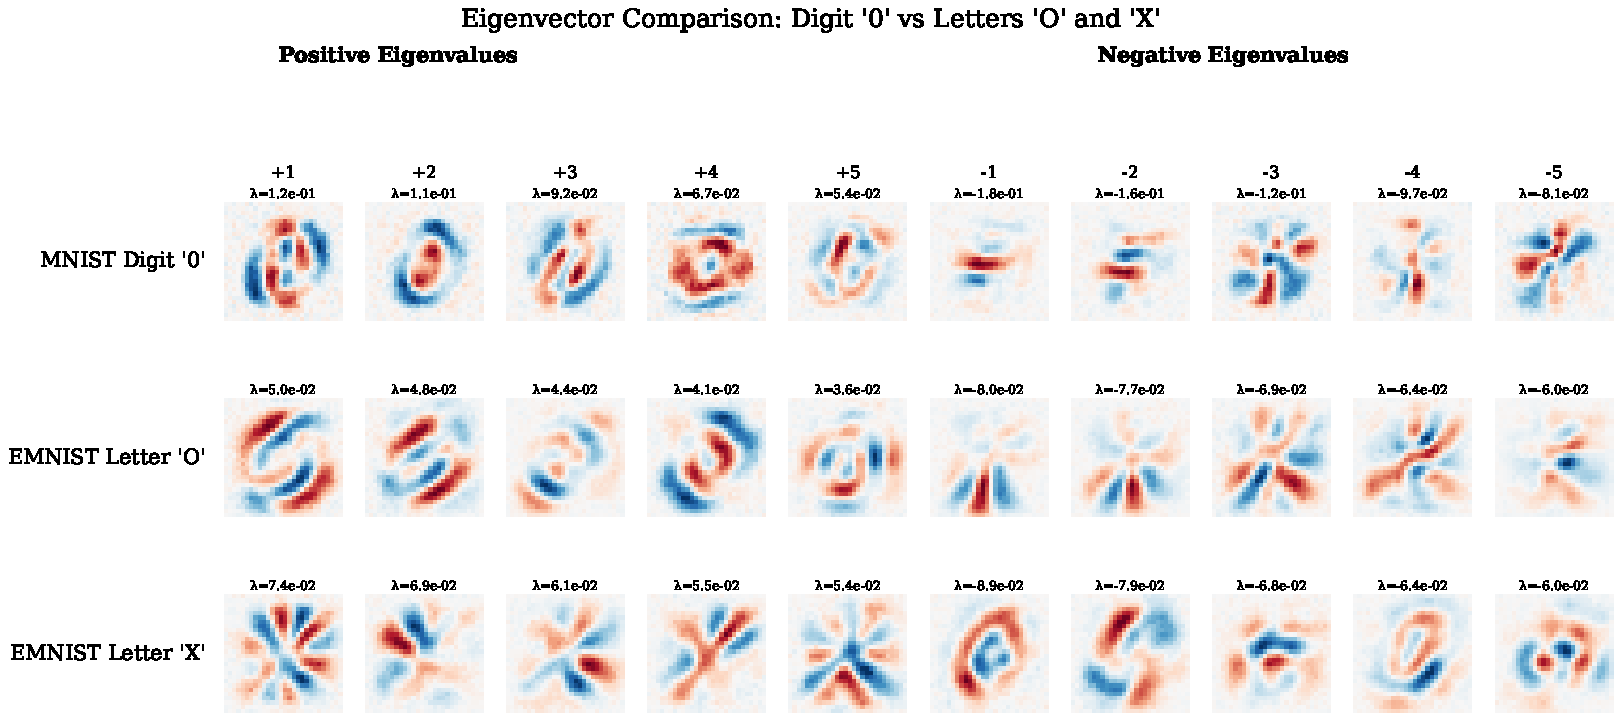
\includegraphics[width=0.9\linewidth]{figures/extension2/extension2_3way_comparison_0_O_X.pdf}
    \caption{Eigenvector comparison: Digit `0' vs Letters `O' (similar) and `X' (dissimilar).
    Visual comparison of top positive and negative eigenvectors for MNIST-0, EMNIST-O, and EMNIST-X.
    The eigenvectors are evidently different across all three classes, suggesting that direct eigenvector alignment may not capture the full structural similarity between geometrically similar classes.}
    \label{fig:3way_comparison}
\end{figure}

To quantify this, we compute the \textbf{maximum absolute cosine similarity} between the top-10 eigenvectors (balanced 5 positive + 5 negative) for:
\begin{itemize}
    \item MNIST ``0'' vs EMNIST ``O'' (geometrically similar: both circular)
    \item MNIST ``0'' vs EMNIST ``X'' (geometrically dissimilar: circular vs crossed lines)
\end{itemize}

Table~\ref{tab:eigenvector_comparison_0_O_X} reports these similarities, averaged over 5 seeds.

\begin{table}[htbp]
\centering
\caption{Absolute Cosine Similarity between Top 10 Eigenvectors (Balanced: 5 Positive + 5 Negative), Mean over 5 seeds}
\label{tab:eigenvector_comparison_0_O_X}
\begin{tabular}{cc|cc}
\toprule
Eigenvector & Eigenvalue & \multicolumn{2}{c}{Maximum Absolute Cosine Similarity} \\
\cmidrule(lr){3-4}
Rank & Sign & MNIST-0 vs & MNIST-0 vs \\
 & & EMNIST-O & EMNIST-X \\
\midrule
1 & + & $0.319 \pm 0.066$ & $0.291 \pm 0.054$ \\
2 & + & $0.596 \pm 0.063$ & $0.725 \pm 0.115$ \\
3 & + & $0.561 \pm 0.048$ & $0.473 \pm 0.073$ \\
4 & + & $0.319 \pm 0.044$ & $0.223 \pm 0.081$ \\
5 & + & $0.390 \pm 0.040$ & $0.262 \pm 0.068$ \\
6 & - & $0.278 \pm 0.052$ & $0.319 \pm 0.087$ \\
7 & - & $0.158 \pm 0.068$ & $0.276 \pm 0.058$ \\
8 & - & $0.336 \pm 0.066$ & $0.316 \pm 0.087$ \\
9 & - & $0.350 \pm 0.117$ & $0.210 \pm 0.066$ \\
10 & - & $0.270 \pm 0.121$ & $0.295 \pm 0.105$ \\
\midrule
\textbf{Mean} & & \textbf{$0.358 \pm 0.026$} & \textbf{$0.339 \pm 0.017$} \\
\bottomrule
\end{tabular}
\end{table}

\textbf{The critical failure}: Cosine similarity \textbf{cannot distinguish} between similar and dissimilar pairs.
The mean similarity for MNIST-0 vs EMNIST-O (geometrically similar) is \textbf{0.358}, while the similarity for MNIST-0 vs EMNIST-X (geometrically dissimilar) is \textbf{0.339}---virtually identical values.
This demonstrates that cosine similarity between eigenvectors fails to capture the geometric relationship between classes.

This failure is systematic across all digit--letter pairs, as shown in Figure~\ref{fig:cosine_similarity_heatmap}.
The heatmap of absolute cosine similarity between MNIST digits and EMNIST letters shows no clear pattern distinguishing geometrically similar pairs (e.g., 0--O, 1--I, 2--Z, 5--S) from dissimilar ones.

\begin{figure}[h]
    \centering
    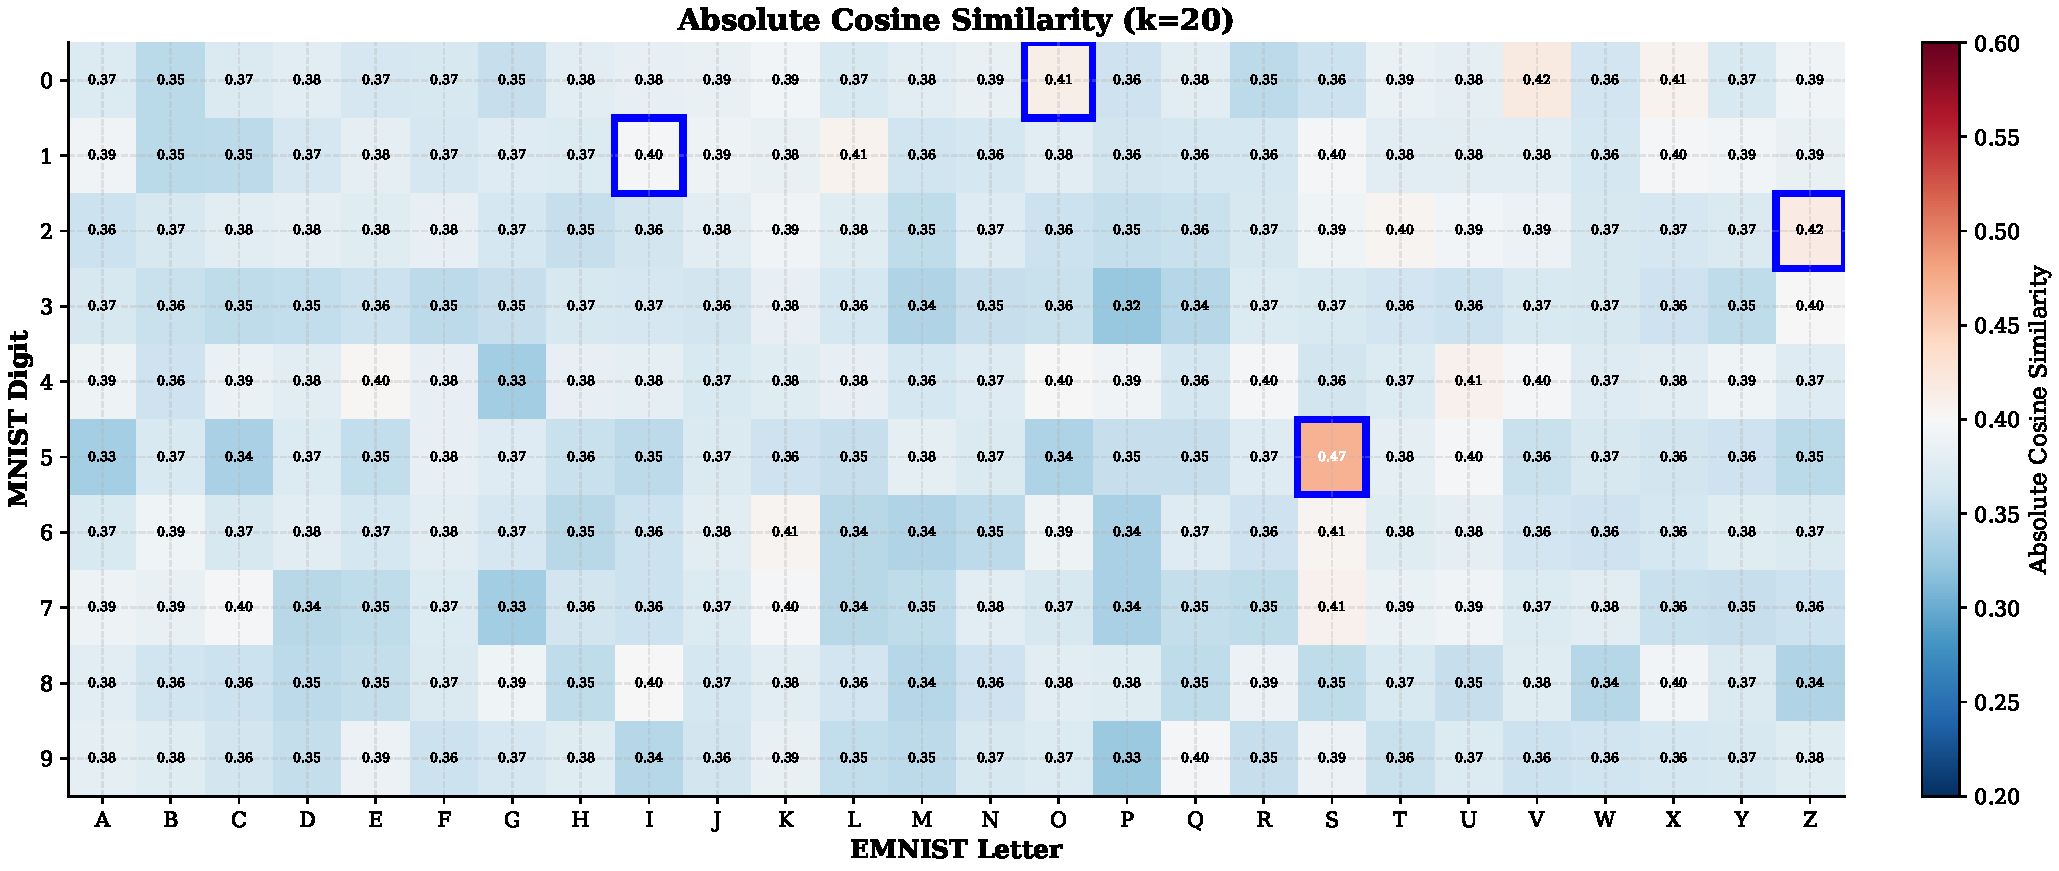
\includegraphics[width=0.8\linewidth]{figures/extension2/extension2_heatmap_abs_cosine_similarity.pdf}
    \caption{Absolute Cosine Similarity between MNIST Digits and EMNIST Letters ($k=20$).
    The heatmap shows no clear pattern distinguishing geometrically similar pairs (expected: bright diagonal-like entries for 0--O, 1--I, 2--Z, 5--S) from dissimilar ones.
    This confirms that cosine similarity between eigenvectors fails to capture geometric relationships.}
    \label{fig:cosine_similarity_heatmap}
\end{figure}

The root cause is that the bilinear eigensystem uses a \textbf{shared eigenvector matrix $V$} and class-specific eigenvalues $\lambda_c$.
Comparing \textbf{only} eigenvectors misses the main source of class information: \textbf{how each class weights those shared directions}.
This motivates a metric that directly compares the full quadratic forms implemented by each class, incorporating both eigenvector alignment and eigenvalue patterns.

\subsection{Method: Quadratic Form Similarity}

To solve the failure of cosine similarity, we need a metric that incorporates \textbf{both} eigenvector alignment and eigenvalue patterns.
For a bilinear MLP, the class-$c$ logit can be written as a \textbf{quadratic form}:
\[
y_c(x) \;=\; x^\top A_c x,\quad A_c = V \,\mathrm{diag}(\lambda_c)\, V^\top.
\]

To compare the \textbf{full decision surfaces} for two classes $A$ and $B$ (possibly from different datasets), we define \textbf{Quadratic Form Similarity}, which directly measures how similar the actual computations performed by each class are:
\[
\mathrm{sim}(A,B) \;=\; 
\frac{\operatorname{tr}(A \cdot B)}{\lVert A \rVert_F \,\lVert B \rVert_F},
\]
which lies in $[-1, 1]$.

For a \textbf{rank-$k$} truncation (using the top $k$ eigenmodes), this can be written in terms of eigenpairs as:
\[
\mathrm{sim}(A,B)
\;=\;
\frac{\sum_{i,j} \lambda_i^A\, \lambda_j^B \,\cos^2(v_i^A, v_j^B)}
{\lVert \lambda^A \rVert_2\, \lVert \lambda^B \rVert_2}.
\]

\textbf{Key properties that solve the cosine similarity problem:}
\begin{itemize}
    \item Incorporates \textbf{both} eigenvector alignment and eigenvalue magnitudes, unlike cosine similarity which ignores eigenvalues.
    \item \textbf{Eigenvalue signs matter}: same-sign directions contribute positively; opposing signs cancel, allowing discrimination between similar and dissimilar pairs.
    \item Measures \textbf{how similar the actual quadratic computations $x^\top A x$} are, not just the span of eigenvectors, enabling it to distinguish geometrically similar classes (e.g., 0--O) from dissimilar ones (e.g., 0--X).
\end{itemize}

\subsection{Results: Quadratic Form Similarity Solves the Discrimination Problem}

In contrast to cosine similarity, which failed to distinguish similar pairs (0--O: 0.358) from dissimilar ones (0--X: 0.339), Quadratic Form Similarity successfully discriminates between geometrically similar and dissimilar digit--letter pairs.
Using Quadratic Form Similarity at $k=20$, we obtain strong quantitative evidence for structural alignment.

Quadratic Form Similarity produces a \textbf{large gap} between similar and dissimilar pairs (0.400 vs -0.060), achieves \textbf{strong statistical significance} ($p < 10^{-4}$), and allows \textbf{negative similarity}, indicating genuinely opposite quadratic structure for dissimilar shapes.
This is visually apparent in the Quadratic Form heatmaps.

For \textbf{MNIST digits vs EMNIST digits} (Figure~\ref{fig:quadratic_form_digits}), the strong diagonal indicates near-identical circuits for the same digit across datasets, confirming that the learned features are writer-independent.

\begin{figure}[h]
    \centering
    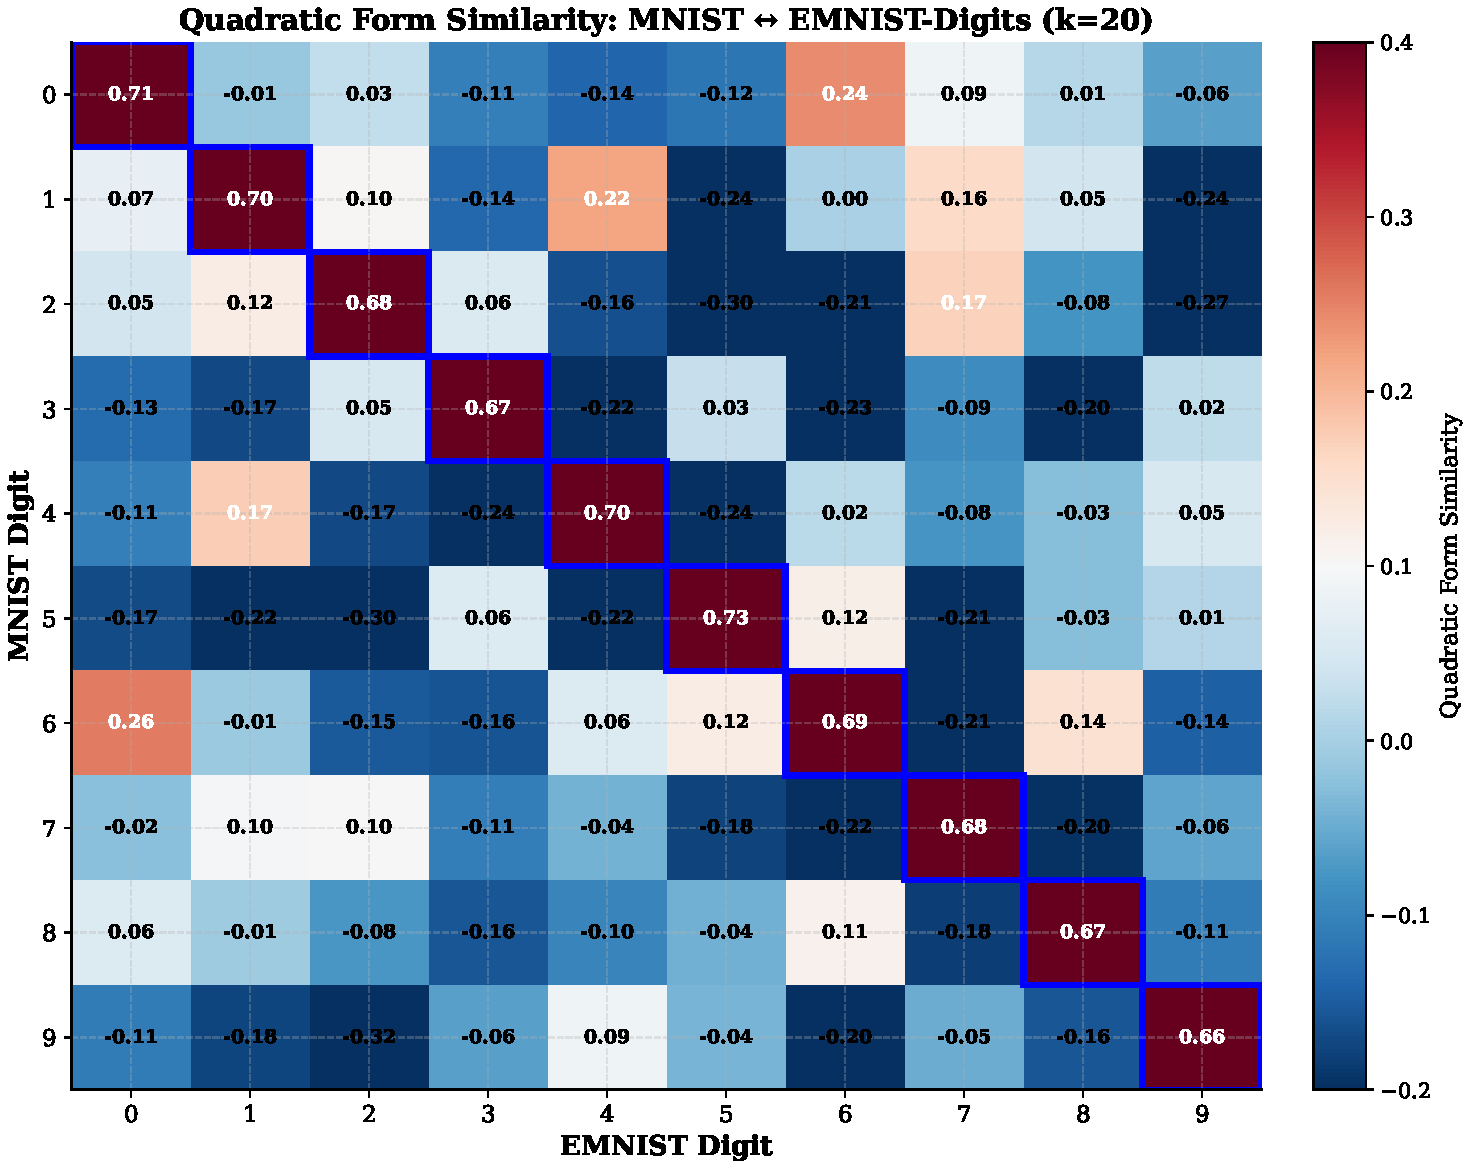
\includegraphics[width=0.8\linewidth]{figures/extension2/extension2_quadratic_form_heatmap_digits.pdf}
    \caption{Quadratic Form Similarity: MNIST Digits vs EMNIST-Digits ($k=20$).
    The strong diagonal indicates near-identical circuits for the same digit across datasets, confirming writer-independent feature learning.}
    \label{fig:quadratic_form_digits}
\end{figure}

For \textbf{MNIST digits vs EMNIST letters} (Figure~\ref{fig:quadratic_form_letters}), bright entries at expected shape-matched pairs (0--O, 1--I, 2--Z, 5--S) indicate mechanistically similar circuits, while unrelated letters remain near zero or negative.
This demonstrates that Quadratic Form Similarity successfully distinguishes geometrically similar pairs from dissimilar ones.

\begin{figure}[h]
    \centering
    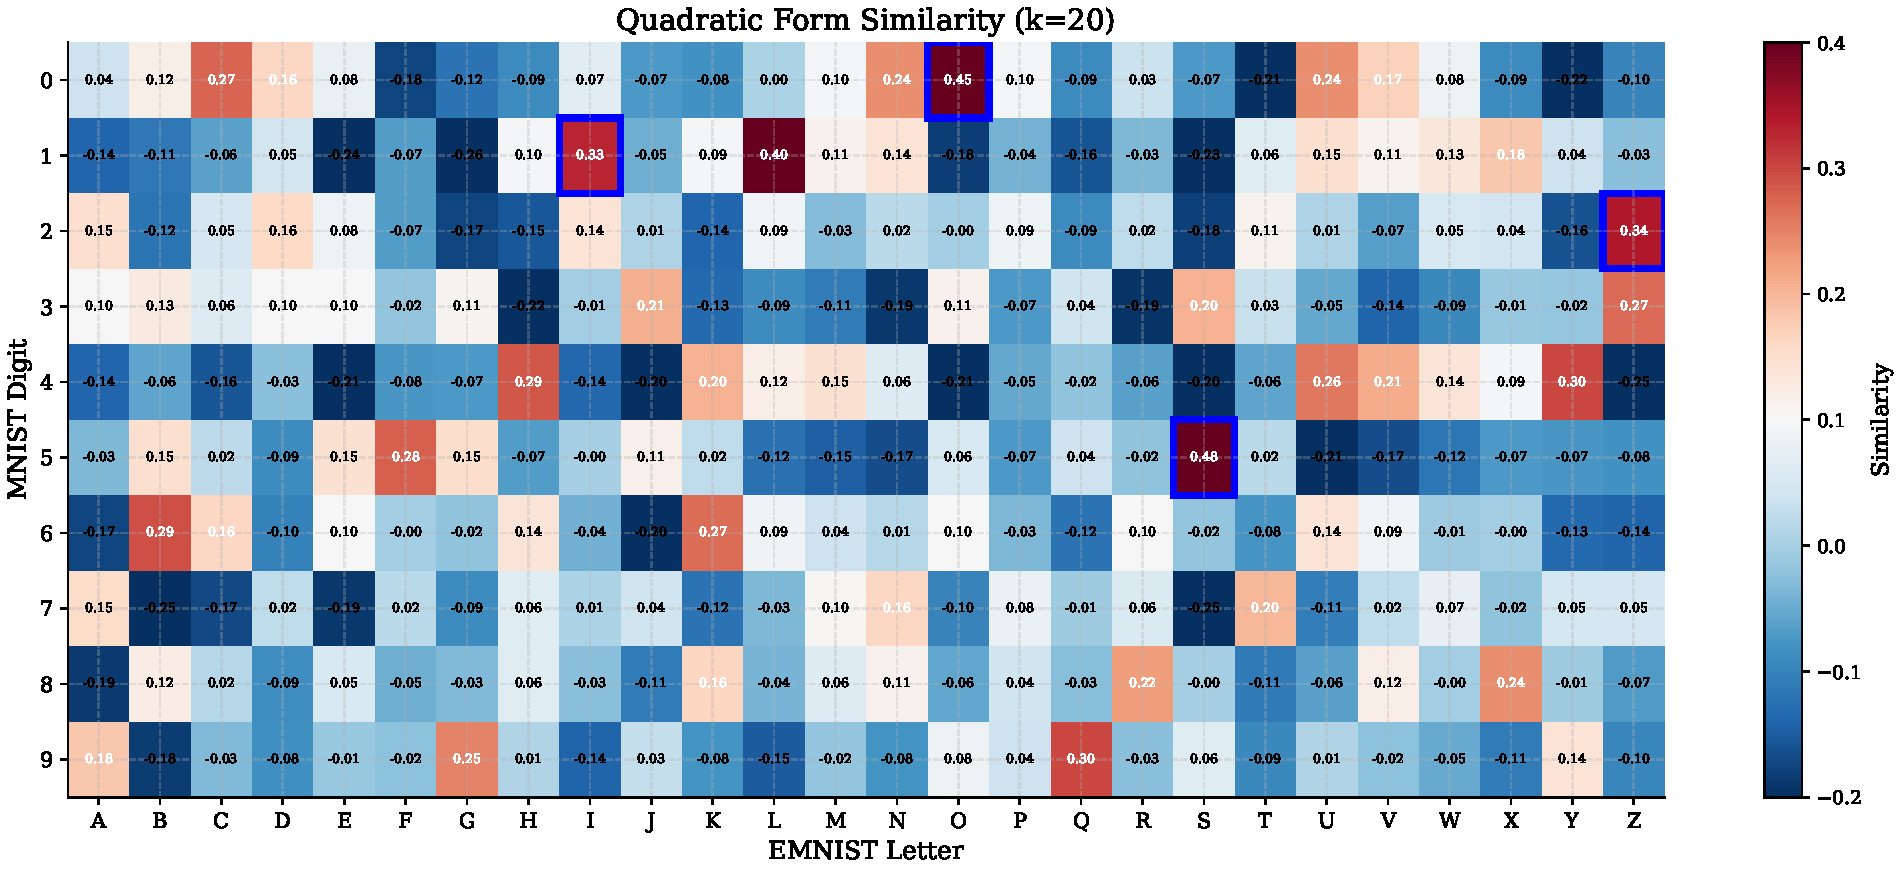
\includegraphics[width=0.8\linewidth]{figures/extension2/extension2_heatmap_quadratic_form.pdf}
    \caption{Quadratic Form Similarity: MNIST Digits vs EMNIST Letters ($k=20$).
    Bright entries at expected shape-matched pairs (0--O, 1--I, 2--Z, 5--S) indicate mechanistically similar circuits, while unrelated letters remain near zero or negative.
    This demonstrates successful discrimination between geometrically similar and dissimilar pairs.}
    \label{fig:quadratic_form_letters}
\end{figure}

\subsubsection{Ranking Analysis}

For each MNIST digit, we rank all 26 EMNIST letters by Quadratic Form Similarity and record the rank of the \textbf{expected} letter:

\begin{table}[h]
    \centering
    \caption{Ranking analysis: Position of expected letter among all 26 EMNIST letters when sorted by Quadratic Form Similarity to each MNIST digit.
    Mean rank of 1.2 (vs random baseline of 13) indicates strong specificity.}
    \label{tab:ranking_analysis}
    \begin{tabular}{lccccc}
        \toprule
        Metric & 0--O & 1--I & 2--Z & 5--S & Mean Rank \\
        \midrule
        \textbf{Quadratic Form} & \textbf{1} & \textbf{2} & \textbf{1} & \textbf{1} & \textbf{1.2} \\
        \bottomrule
    \end{tabular}
\end{table}

\begin{itemize}
    \item \textbf{3/4 pairs} rank \textbf{\#1} out of 26 letters.
    \item The remaining pair ranks \textbf{\#2}.
    \item A random baseline would be rank $\sim$13.
\end{itemize}

The \textbf{similarity-vs-$k$} plot (Figure~\ref{fig:similarity_vs_k}) shows that as we increase the number of eigenvectors $k$, similarity for shape-matched pairs \textbf{increases and converges} around $k=20$, while dissimilar pairs stay near zero or negative throughout, with non-overlapping 90\% confidence intervals across most of the range.

\begin{figure}[h]
    \centering
    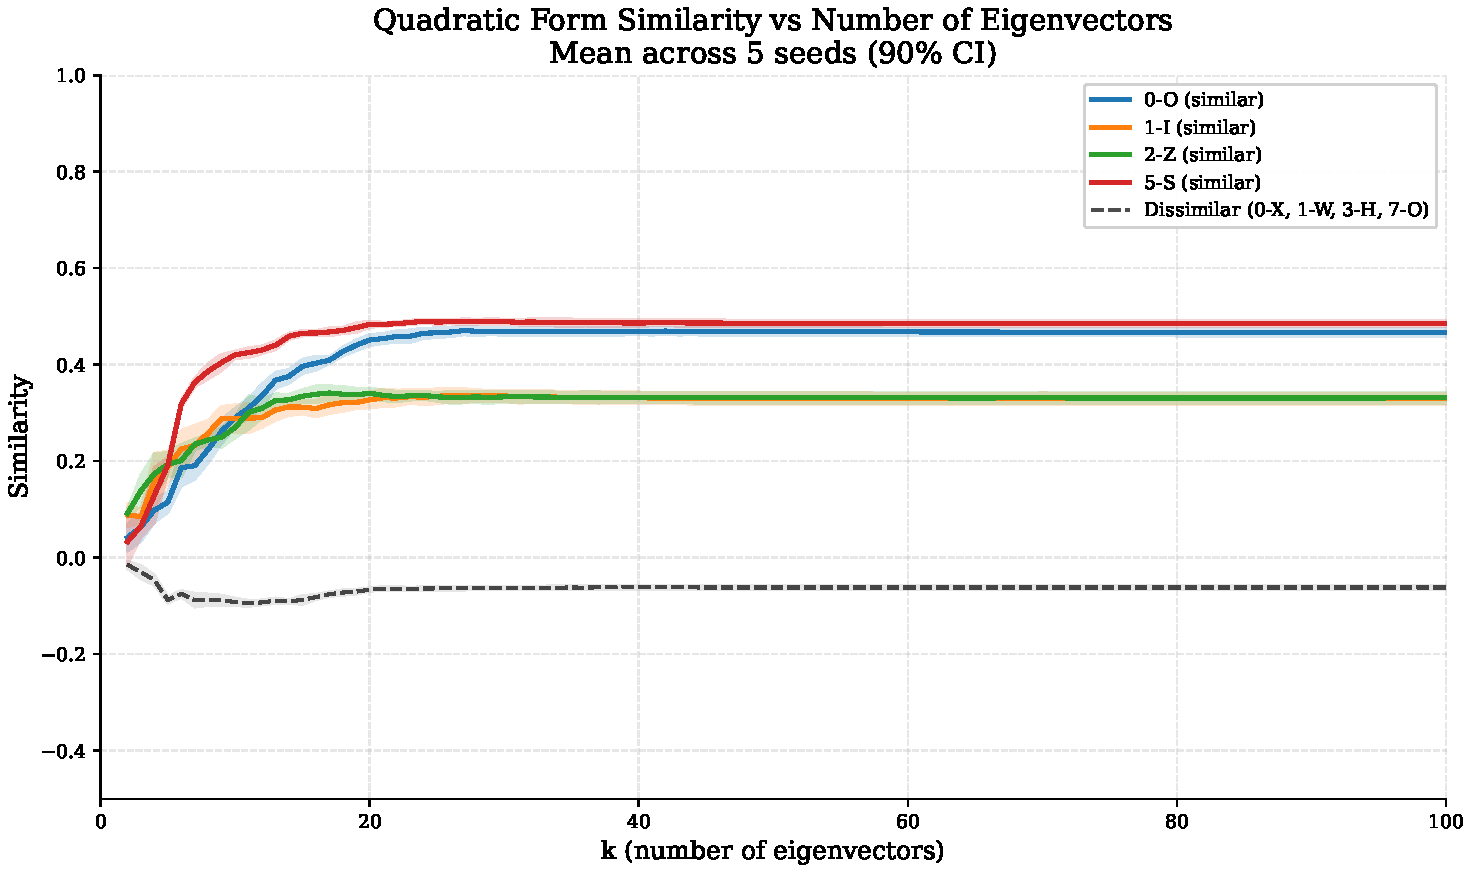
\includegraphics[width=0.8\linewidth]{figures/extension2/extension2_similarity_vs_k_quadratic_form.pdf}
    \caption{Quadratic Form Similarity vs number of eigenvectors $k$.
    Mean across 5 seeds with 90\% CI.
    Similar pairs (top lines) increase and converge around $k=20$, while dissimilar pairs (bottom lines) remain near zero or negative throughout.
    The convergence indicates that the top-$k$ approximation captures the full geometric correspondence.}
    \label{fig:similarity_vs_k}
\end{figure}

This indicates that \textbf{additional eigenmodes up to $k \approx 20$ consistently reinforce the same geometric correspondence}, and the convergence suggests that the top-$k$ approximation captures the essential structure without being washed out by higher-order noise.

\subsection{Conclusion: Evidence for Universal Geometric Circuits}

In this extension, we test whether the interpretability seen in Section~\ref{sec:reproduction} is a \textbf{MNIST-only artifact} or reflects genuinely \textbf{universal geometric structure}.
Our findings support the latter:

\textbf{Functionally}, \textbf{regularized CoM-based} Bilinear MLPs:
\begin{itemize}
    \item Maintain \textbf{writer-independent} performance across MNIST $\leftrightarrow$ EMNIST-Digits ($\sim$97.7\% bidirectional accuracy).
    \item Substantially improve \textbf{domain transfer} to USPS (from $\sim$53\% to $\sim$72\% accuracy).
    \item Exhibit \textbf{geometry-aware semantic confusion}, mapping letters O/I/Z/S to digits 0/1/2/5 with high per-letter accuracy and \textbf{perfect} correctness at the level of which digit each letter is mapped to.
\end{itemize}

\textbf{Mechanistically}, \textbf{Quadratic Form Similarity} shows that:
\begin{itemize}
    \item The \textbf{digit ``0'' circuit} in a MNIST model is mathematically almost identical to the \textbf{``O'' circuit} in an EMNIST-letter model, with similar results for 1--I, 2--Z, and 5--S.
    \item Similar pairs are sharply separated from dissimilar ones (0.400 vs -0.060, $p < 0.0001$), with expected letters ranking at the very top among all 26 options (mean rank 1.2).
\end{itemize}

These results argue that the bilinear models, especially under CoM and regularization, learn \textbf{stable, transferable geometric forms} that generalize across datasets, resolutions, and even alphabets.
This strengthens the transparency claim of the paper: the weight-based features we interpret in Section~\ref{sec:reproduction} are \textbf{not hallucinations or MNIST-specific quirks}, but \textbf{mechanistically robust circuits} that capture genuinely reusable shapes.

